\documentclass[crop,tikz,multi=my]{standalone}

\usetikzlibrary{decorations.pathreplacing,positioning,calc,intersections,3d,shapes.geometric,math}

\begin{document}

\newcommand{\SolveLadder}{
		\coordinate (Om1) at (0,0);
		\coordinate (Om2) at (3,0);
		\foreach \x in {1,2,3} {\coordinate (Om1\x) at (0,\x);
							\coordinate (Om2\x) at (3,\x);}
	   	\node[below] at (Om1) {$\Omega_1$};
	 	\node[below] at (Om2) {$\Omega_2$};
		\draw[very thick,black] (Om1) -- (Om2);
}

\begin{my}
	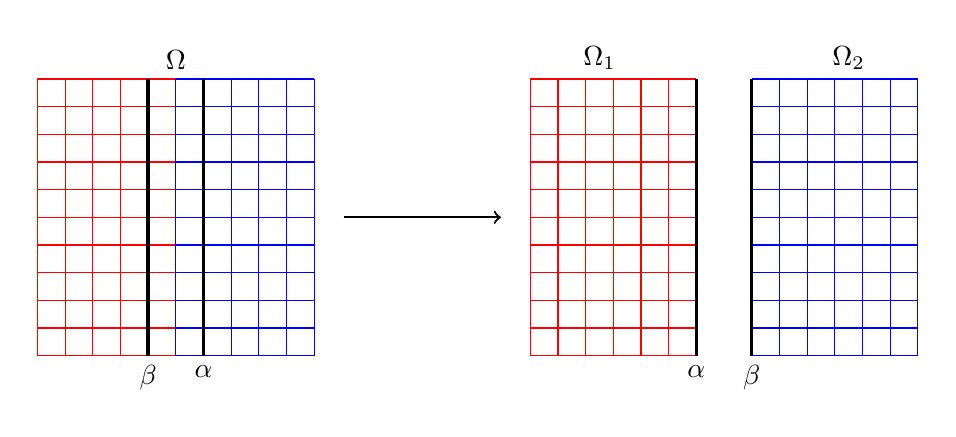
\begin{tikzpicture}
		\matrix[row sep=1em, column sep=1em]{
%			\draw[step=1em,black] (0,0) grid (10em,10em);
			\draw[step=1em,red] (0,0) grid (5em,10em);
			\draw[step=1em,blue] (5em,0) grid (10em,10em);
			\node[below] at (6em,0) {$\alpha$};
			\draw[very thick, black] (6em,0) -- (6em,10em);
			\node[below] at (4em,0) {$\beta$};
			\draw[very thick, black] (4em,0) -- (4em,10em);
			\node[above] at (5em,10em) {$\Omega$};
			& \draw[thick,black,->] (0,5em) -- (2,5em); &
			\draw[step=1em,red] (0,0) grid (6em,10em);
			\draw[step=1em,blue] (8em,0) grid (14em,10em);
			\node[below] at (6em,0) {$\alpha$};
			\node[below] at (8em,0) {$\beta$};
			\draw[very thick, black] (6em,0) -- (6em,10em);
			\draw[very thick, black] (8em,0) -- (8em,10em);
			\node[above] at (2.5em,10em) {$\Omega_1$};
			\node[above] at (11.5em,10em) {$\Omega_2$};
		\\};
	\end{tikzpicture}
\end{my}

\begin{my}
	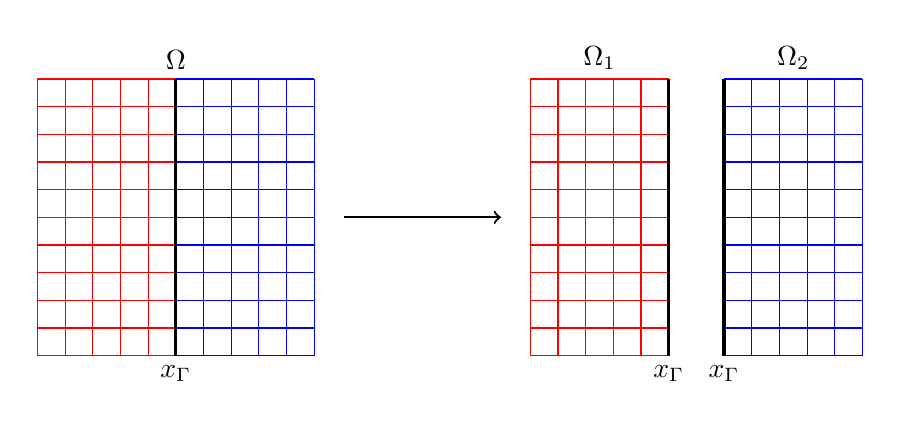
\begin{tikzpicture}
		\matrix[row sep=1em, column sep=1em]{
%			\draw[step=1em,black] (0,0) grid (10em,10em);
			\draw[step=1em,red] (0,0) grid (5em,10em);
			\draw[step=1em,blue] (5em,0) grid (10em,10em);
			\node[below] at (5em,0) {$x_\Gamma$};
			\draw[very thick, black] (5em,0) -- (5em,10em);
			\node[above] at (5em,10em) {$\Omega$};
			& \draw[thick,black,->] (0,5em) -- (2,5em); &
			\draw[step=1em,red] (0,0) grid (5em,10em);
			\draw[step=1em,blue] (7em,0) grid (12em,10em);
			\node[below] at (5em,0) {$x_\Gamma$};
			\node[below] at (7em,0) {$x_\Gamma$};
			\draw[very thick, black] (5em,0) -- (5em,10em);
			\draw[very thick, black] (7em,0) -- (7em,10em);
			\node[above] at (2.5em,10em) {$\Omega_1$};
			\node[above] at (9.5em,10em) {$\Omega_2$};
		\\};
	\end{tikzpicture}
\end{my}

\begin{my}
	\begin{tikzpicture}
			\SolveLadder
			\draw[black, ->] (Om1) -- (Om21) -- (Om12) -- (Om23);
			\draw[black, ->] (Om2) -- (Om11) -- (Om22) -- (Om13);
			\draw[decorate,decoration={brace,mirror,amplitude=4pt,raise=6pt},blue] (Om21) -- node[right=8pt] {$\Delta T_2^2$} (Om22);
			\draw[decorate,decoration={brace,amplitude=4pt,raise=6pt},blue] (Om12) -- node[left=8pt] {$\Delta T_1^2$} (Om13);
	\end{tikzpicture}
\end{my}

\begin{my}
	\begin{tikzpicture}
			\SolveLadder
			\draw[black, ->] (Om1) -- (Om21) -- (Om12) -- (Om23);
			\draw[black, ->] (Om2) -- (Om11) -- (Om22) -- (Om13);
			\draw[decorate,decoration={brace,mirror,amplitude=4pt,raise=6pt},blue] (Om21) -- node[right=8pt] {$\Delta T_2^2$} (Om22);
			\draw[decorate,decoration={brace,amplitude=4pt,raise=6pt},blue] (Om11) -- node[left=8pt] {$\Delta T_1^2$} (Om12);
			\draw[decorate,decoration={brace,mirror,amplitude=4pt,raise=6pt},blue] (Om22) -- node[right=8pt] {$\Delta T_2^3$} (Om23);
			\draw[decorate,decoration={brace,amplitude=4pt,raise=6pt},blue] (Om12) -- node[left=8pt] {$\Delta T_1^3$} (Om13);
	\end{tikzpicture}
\end{my}
	
\end{document}